\section{Requirements}
\label{sec:requirements}
Before the search for suitable protocols starts, it is important to know what kind of protocol would suffice and what specification should at least be required. 
This will drastically increase the process of narrowing the search to a handful available protocols. For example in case the line rate is not sufficient, it is immediately clear the protocol is not suited for the application it has to fulfill.

This section contains these requirements with their description and explanation in case this has not been discussed in the previous section. There is a minimum line rate that should be possible to reach. At that rate a certain line range should be covered and flow control has to be included. Error detections and corrections like the Cyclic Redundancy Check and Forward Error Correction are a very important addition to the protocol and their priority will be discussed.

In addition to these requirements it is the purpose to look for a protocol that transfers data in a serial way and not in parallel. Of course bonding could be implemented but this should only apply in case a single line could at least transmit the minimum amount of data required.

\subsection[Line rate target]{Line rate target \hfill OSI Layer 1}
Line rate is the physical speed at which the device communicates with the equipment directly. For this project it has been specified the line rate has to be about 10 Gbps. This results is a rate of 1,25 GB/s when converted to bytes.

However while the line rate is the physical speed, this doesn't mean the actual data (payload) will also be transported at this rate. There is also overhead that has to be taken into account which adds additional information transmitted. The encoding and framing of data to be transmitted have a big impact on the amount of overhead. Error correction will also play a determining factor because this often adds redundant data.
In this case the payload the data contains has to be more than 70\%. This means that a maximum of 30\% overhead is allowed, which still is quite a large percentage.\\

\subsection[Range distance coverage]{Range distance coverage \hfill OSI Layer 1}
This is the effective distance that can be covered by the signal that is carrying the data. In this project it has been specified the data stream should cover short to medium distances that vary between around 10 and 200 m, which corresponds to normal distances covered by cables in data centers.

The range largely depends on the transmission medium, the encoding used by the protocol and how many parallel transmission lines are used. Also the EMI induced on the line by other operating devices or transmission lines can cause the range to decrease. This can be solved by implementing FEC as explained in section \ref{sec:FEC}. Each protocol has it's own effective range distance coverage which makes some protocols very suitable to use in this case while others can quickly be skipped.

\subsection[Forward Error Correction]{Forward Error Correction \hfill OSI Layer 1}
Forward Error Correction is an optional feature but as explained the addition could prove very useful. Especially in noisy environments this could prevent a lot of possible errors. Especially since it provides the ability to also correct these. It is certainly a feature to keep in mind and it would be great if a protocol provides at least the must haves and also has implemented FEC.

\subsection[Flow control]{Flow control \hfill OSI Layer 2}
Implementing flow control is a must have so it's absolutely necessary that the chosen or designed protocol includes this feature. Flow control is the ability to manage the data rate of the transmission process between two devices. While the transmitter cant send data at the maximum speed the transceiver and protocol are allowing, this doesn't mean the receiver can always process all this data at the same rate. For example the receiver could have other tasks or the FIFO is read out at a slower rate and has the tendency to overflow, this could cause data loss because the receiver is simply overwhelmed by the amount of data and has no place to store it. The consequences could be disastrous.

By implementing flow control the receiver will be added the ability to make it's processing speed clear to the transmitter. There are multiple variants to implement this but now the transmitter has an indication at which rate it can send data. The most simple way is Stop and Wait which is depicted in Figure~\ref{fig:Flow_Control}~\cite{FlowControl}. The disadvantage of this way is the waiting time before the ACK arrives at the transmitter and this wastes resources. A different approach is the Sliding Window in which multiple frames are transmitted and while transmitting the ACK's will arrive. This boosts the efficiency considerably. \\

\begin{figure}[H]
	\centering
	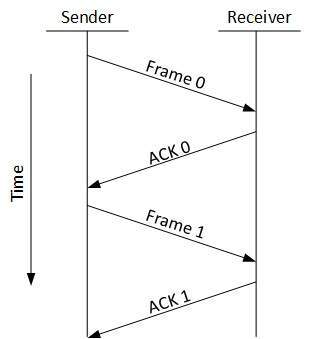
\includegraphics[width=0.3\textwidth]{stop_and_wait.jpg}	
	\caption{The simple Stop and Wait implementation of flow control.}
	\label{fig:Flow_Control}
\end{figure} 

\subsection[Cyclic Redundancy Check]{Cyclic Redundancy Check \hfill OSI Layer 2}
The Cyclic Redundancy Check is an optional way of error detection which is used to detect corruption in the received frames. This is not a must have but it would be very useful if a protocol meeting the minimum requirements would also offer this feature. It would cause frame errors to be detected and prevent using corrupt data as if it were identical to the transmitted data.


\subsection[Channel bonding]{Channel bonding \hfill OSI Layer 3}
This is a technique where two or more links are combined to increase throughput or to add redundancy. Differently formulated this will lead to an increase in the total amount of bandwidth available. For example this technique can often be found in wireless Internet connections like 4G and WiFi. Figure~\ref{Fig:Bonding} shows a visualization of the bonding technology~\cite{Bonding_Image}.

Especially in the case of using FPGA's this technique comes in very useful since it offers the possibility to bond multiple transceivers and can handle the high speeds at which data flows. Xilinx and Altera for example both offer their own specific high speed transceivers which individually can reach high line rates but they can be bonded for even higher rates. Bonding is a completely optional feature to add but as explained this could cause a huge increase in the maximum amount of data that could be transported. This would also make the protocol better suitable for more use in the future.

\begin{figure}[H]
	\centering
	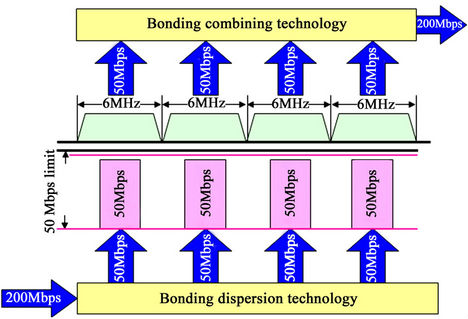
\includegraphics[width=0.6\textwidth]{Bonding.jpg}	
	\caption{Transmitting data over different channels using bonding.}
	\label{Fig:Bonding}
\end{figure} 

Not only does bonding provide higher bandwidth, the distance that can be reached while using wires also extends. The data packets will be fragmented and transmitted containing additional headers~\cite{Bonding_Altera}. This will cause the receiver to be able to reconstruct the complete package using the headers containing crucial information.

Of course implementing this technique requires a lot more effort. All lines will have to be in constant synchronization, otherwise reconstructing packets will be very difficult and the chance is fairly high a lot of data will be lost.
\newpage